\section{Introduction}%Problems regards to discrimination in IC
\label{sec:intro}
	\begin{figure}[t]
		\centering
		\vspace{-10pt}
		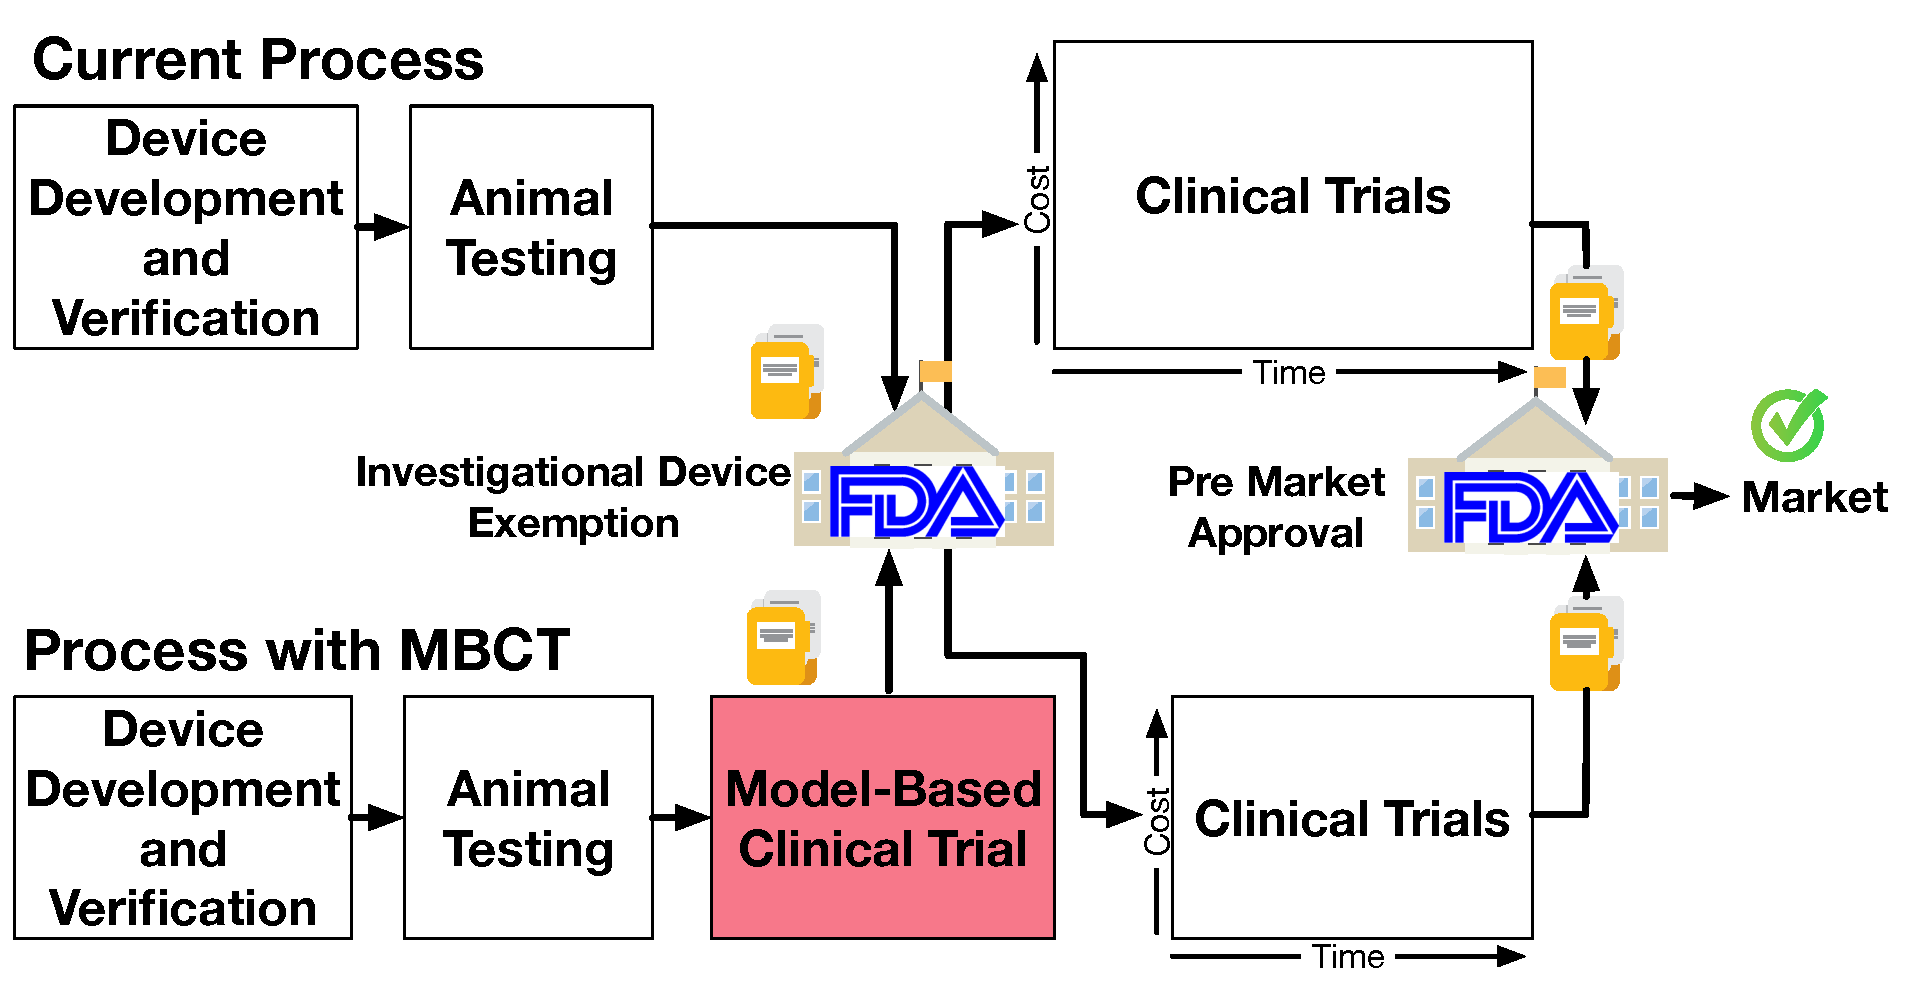
\includegraphics[scale=0.25]{figures/figTransResearchSpectrum.pdf}
		\vspace{-10pt}
		\caption{\small Bringing a device to market.
			Clinical trials are the last step before a new device's market approval.
			Model-based clinical trials will provide insight during planning and execution of clinical trials, leading to reduction in costs and increasing the chance of a successful trial.}
		\vspace{-10pt}
		\label{fig:spectrum}
	\end{figure}
	
The lives of millions of patients around the world depend on medical devices.
In the domain of cardiac devices, for example,
10,000 people in the U.S. receive an Implantable Cardioverter Defibrillator (a heart rhythm adjustment device) every month \cite{asktheicd}.
Clinical trials have presented evidence that patients implanted with ICDs have a mortality rate reduced by up to 31\% \cite{maditrit}.
Unfortunately, ICDs suffer from a high rate of \emph{inappropriate therapy}, which takes the form of unnecessary electric shocks or pulse sequences delivered to the heart.
Inappropriate therapy increases patient stress, reduces their quality of life, and is linked to increased morbidity \cite{shock_mortality}.
Depending on the particular ICD and its settings, the rates of inappropriate therapy range from 46\% to 62\% of all delivered therapy episodes \cite{GoldABBTB11_RIGHTresults}.
\mynote{SD}{This percentage is too high. Inappropriate therapies are typically not more than 20\%.\newline
	HA: this was calculated from RIGHT results. Another figure we could quote is Reported rates of inappropriate therapy range from 11 to 41\% (cited in RIGHT 2006).
	}
The closed loop formed by the organ (heart) and device (ICD) is an example of a life-critical Cyber-Physical System (CPS): the device's software is the cyber component, and the physiological phenomenon (e.g., cardiac rate and electrical activity) is the physical component.
%\headline{The technology in some of these devices combines hardware and software, each of which must be rigorously verified to be efficacious and safe.}
%\headline{In this paper we are concerned with \emph{closed-loop devices}.}
%Such a device is in a feedback loop with the organ(s) it effects (see Fig.\ref{fig:pacemaker}): an ICD for example monitors the heart rate, and delivers therapy to maintain an adequate rate.
%Another example is the artificial pancreas, which monitors blood glucose levels and delivers insulin to maintain safe glucose levels.

\emph{After the verification and testing effort is completed}, regulatory agencies like the F.D.A. require that the safety and efficacy of new devices be demonstrated in a \emph{\ac{CT}} (Fig.~\ref{fig:spectrum}).
%\footnote{In this paper, we always mean a randomized controlled trial, which is the type of trial described here.}
In a trial, a group of patients that are treated with the new device (this is the `intervention group') are compared to a group of patients who are treated with the current standard of care (e.g., a different device currently on the market; this is the `control group').
The objective is to see whether the different devices result in significantly different effects on the patients.
Clinical trials are major endeavors, involving physicians, patients, statisticians, clinical centers, companies and regulators, sometimes in several countries.
Late-phase trials can run for several years, and cost millions of dollars.
For example, a 2002 trial for stents lasted 2 years, enrolled 800 patients and cost \$10 to \$12 million and lasted 24 months \cite{Kaplan04_Cost}.
Trials also pose an inherent risk to the patients in the intervention group by exposing them to an unproven device.
Thus it is crucial that they be well planned, and rigorously executed.

In reality, any trial runs the risk of errors during its planning and execution stages, which can invalidate the results of the trial.
In this paper, we pose and propose an answer to the following question: \emph{how can modeling of CPS assist in the planning and execution of a clinical trial, so as to increase the chances of a successful trial}?
%The advent of computer models for various physiological functions defines a new convergence point for computer science and engineering with medicine.

Specifically, in this paper,
we demonstrate how  computer models can be used for early, affordable and reproducible testing of a clinical trial's premises and assumptions.
Model-based empirical validation of the premises reduces the risk of conducting a trial that fails to demonstrate the desired effect (typically, an improvement of new intervention over the control). 
We used the Rhythm ID Going Head to Head Trial (RIGHT) \cite{GoldABBTB11_RIGHTresults}, which lasted five years and sought to compare the diagnostic algorithms used by two ICDs for correctly diagnosing potentially fatal tachycardias (abnormally fast heart rhythms).
Our contributions are as follows:
\begin{itemize}
	\item We defined a heart model capable of producing several types of tachycardias, in terms of both timing characteristics and morphology of the electrical signals (the \emph{\acp{EGM}})
	(Section \ref{sec:heart modeling}).
	This model allows us to generate thousands of arrhythmia exemplars which serve as our virtual trial patients.
	\item For modeling purposes, we annotated segments of over 100 \ac{EGM} records of real patients to extract the tachycardias that they suffered from at time of recording.
	These electrograms are essential to simulate our models.
	\item Using the openly available literature, we implemented the tachycardia detection algorithms of two major ICD manufacturers: Boston Scientific and Medtronic.
	(See Section \ref{sec:device models}).
	\item We developed an experimental setup to validate our implementation of the Boston Scientific algorithm against a real ICD (Section \ref{sec:validation}).
	\mynote{SD}{wants "against a real ICD" deleted..}
	
	The connected heart model and ICD form the CPS under study.
	\item With the above elements in place, we generated a synthetic cohort, consisting of $11,000+$ heart models displaying a wide range of tachycardias.
	These models are then connected to the 2 ICD implementations and arrhythmia detection results are recorded.
	This allows us to estimate their relative efficacy on an condition-by-condition basis
	(Section \ref{sec:results}.)
\end{itemize}

We call our approach \ac{MBCT}, or \ac{MBCT}.
An \ac{MBCT} is a trial whose subjects are computer models of the (heart, device) closed-loop system.
By generating large cohorts, we can answer several questions contributing to the planning and execution of a clinical trial.

\paragraph{Modeling as regulatory grade evidence}
\label{sec:related work}
Most medical models today are aimed at either better understanding the phenomenon under study \cite{vfiborganization_Tusscher07} or at device debugging and verification \cite{VHM_proc}. 
There is only one case in which a computer model has been used to intervene in the regulatory process of medical devices, namely the T1 Diabetes Model (T1DM) of UVA/PADOVA \cite{T1DM}.
T1DM models glucose kinetics in hypoglycemia, and has been accepted by the FDA as a substitute for animal trials.
The T1DM has a fixed virtual cohort with 300 patients.
Its objective is to test the efficacy of new glucose control algorithms by simulating them on the virtual cohort.
While our models can be used in this way, our objective here is to target specific clinical trials steps and improve how they are conducted.
This dictates the experimental setup and the cohort generation considerations.

The Avicenna consortium \cite{Avicenna} lays out a vision for `In-Silico Clinical Trials' similar to our approach.
However, the emphasis in Avicenna is on individualized patient models, as they propose to customize the model to each patient enrolled in a trial.
In the present work, we propose a usage of MBCT \emph{prior} to recruitment.
Thus our models need not be fitted to a given patient's data, which might be impossible, invasive, or burdensome for the conduct of the trial.


\begin{figure}[tb]
	\vspace{-10pt}
	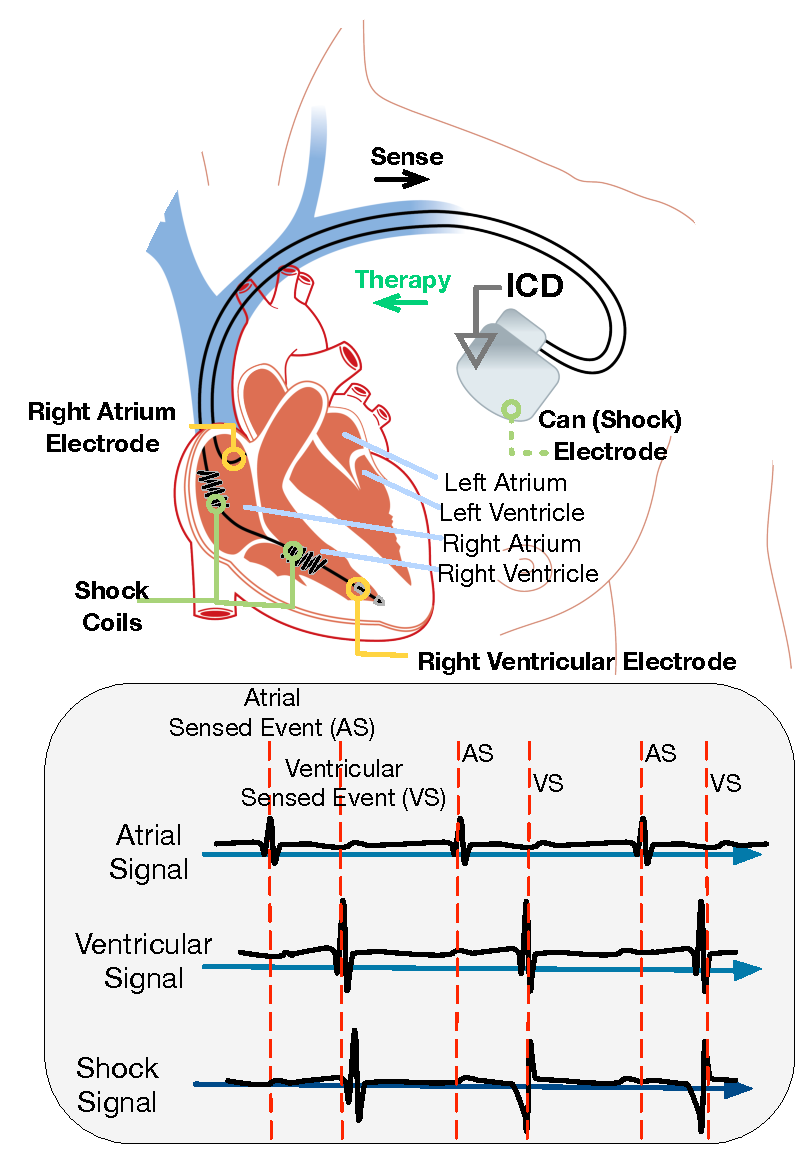
\includegraphics[scale=0.4]{figures/figICD.pdf}
	\vspace{-10pt}
	\smallcaption{ICD connected to the heart. The atrial, ventricular, and shock electrogram signals are measured by the device, which uses them to diagnose the current state of the heart and determine whether therapy is required.}
	\vspace{-10pt}
	\label{fig:icd}
\end{figure}



\begin{figure*}[tb]
	\vspace{-10pt}
	\centering
	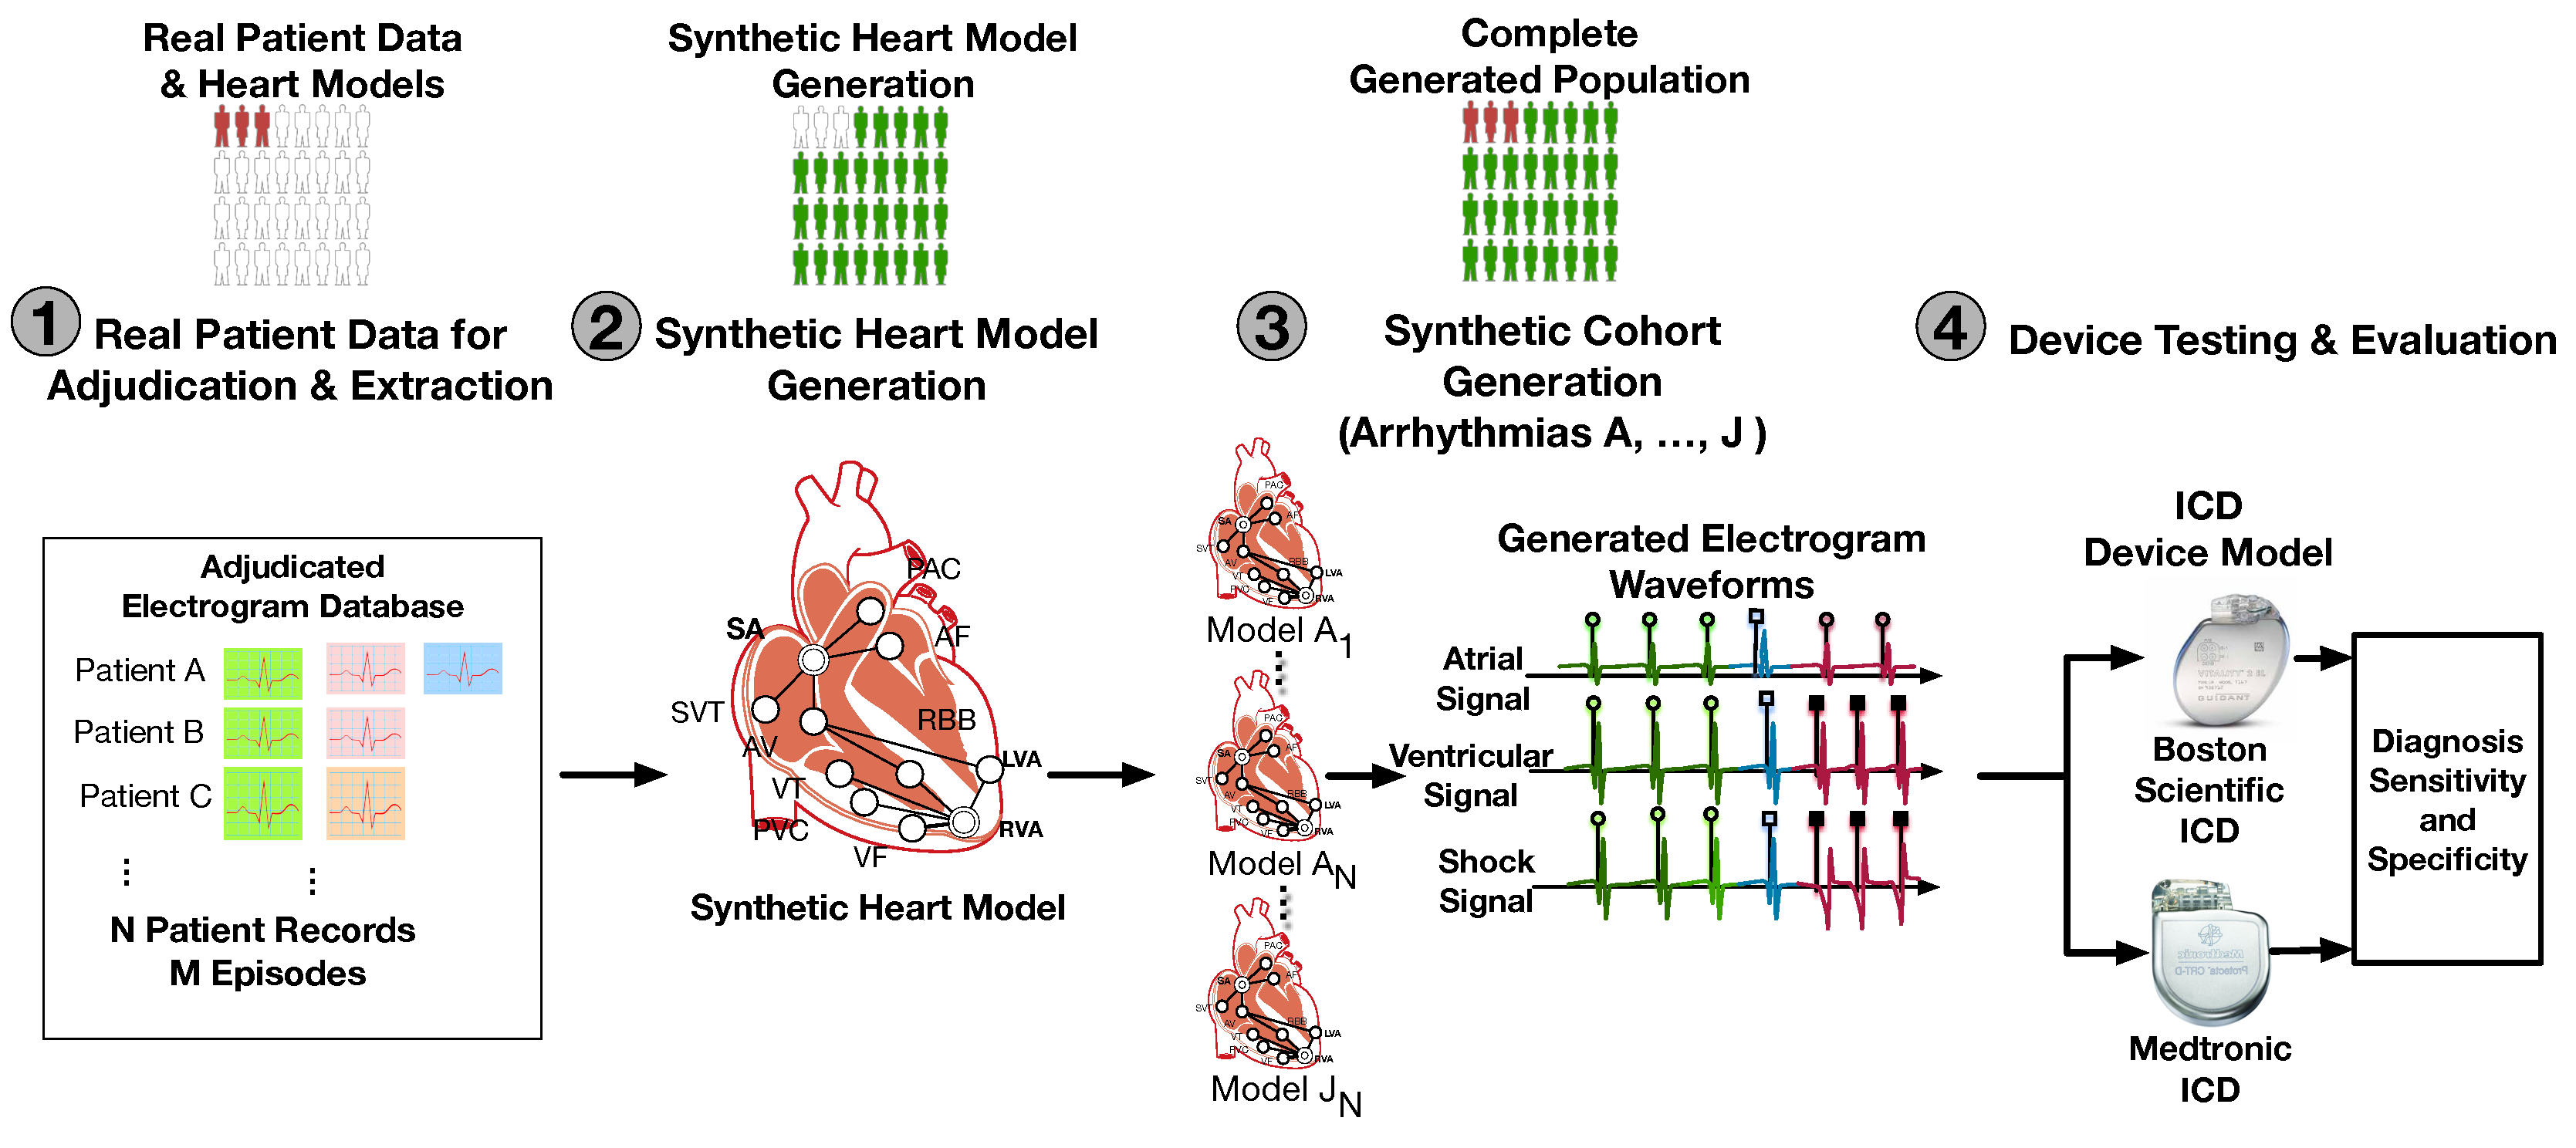
\includegraphics[scale=0.3]{figures/figMBCToverview}
	\vspace{-10pt}
	\caption{Overview of an \ac{MBCT}. 1) \ac{EGM} recordings of real patients are adjudicated to create a table of \ac{EGM} morphologies of various tachycardias. 2) Subsets of these morphologies are combined with a timing model to create a synthetic heart model. 3) Through variation of the parameters of the model, an entire synthetic cohort is generated and simulated to produce synthetic \ac{EGM} signals. 4) Various device evaluation experiments can be executed with this synthetic cohort.}
	\vspace{-10pt}
	\label{fig:mbct overview}
\end{figure*}

